\documentclass{article} % For LaTeX2e
\usepackage{nips13submit_e,times}
%\usepackage{hyperref}
\usepackage[round]{natbib}
\usepackage{url}
\usepackage{float}
\usepackage{graphicx}
\usepackage{amsmath, amssymb}
\usepackage{comment}
%\documentstyle[nips13submit_09,times,art10]{article} % For LaTeX 2.09

\title{Incremental SVD for large-scale recommendation algorithms}

\author{
Stephen Merity
\And
J. Benjamin Cook
}

% The \author macro works with any number of authors. There are two commands
% used to separate the names and addresses of multiple authors: \And and \AND.
%
% Using \And between authors leaves it to \LaTeX{} to determine where to break
% the lines. Using \AND forces a linebreak at that point. So, if \LaTeX{}
% puts 3 of 4 authors names on the first line, and the last on the second
% line, try using \AND instead of \And before the third author name.

\newcommand{\fix}{\marginpar{FIX}}
\newcommand{\new}{\marginpar{NEW}}
\newcommand{\A}{\mathbf{A}}
\newcommand{\T}{\textrm{T}}

\nipsfinalcopy % Uncomment for camera-ready version

\begin{document}

\maketitle

\begin{abstract}
Singular value decomposition (SVD) is fundamental to many machine learning algorithms, primarily being used for dimensionality reduction.
Unfortunately, SVD algorithms typically have cubic complexity and require random access to the complete data set, making them impractical for many real world tasks.
We investigate the convergence properties of incremental singular value decomposition (SVD) which does not require the complete data set to be stored in memory.
We then compare this with a traditional, full SVD algorithm to see the impact on orthogonality of the resulting SVD.
To motivate incremental SVD in the context of machine learning, we construct a recommendation system and show the performance of SVD compared to incremental SVD, showing the potential to incrementally build SVD-based models and produce a highly scalable recommendation system.
\end{abstract}

\section{Introduction}

Recommendation systems aim to recommend an item to interested potential customers, tailoring the choice of item based upon both that customer's history and the history of other users.
The items recommended can be divserse, including movies, music, web pages, or other general products.
These systems have evolved from novelties to vital tools that are re-shaping the world of e-commerce.
By learning from both the customer and the broader community as to which items should be recommended to someone, these successful recommendations can lead to substantial improvements in both revenue and customer satisfaction \citep{schafer1999recommender}.

Within recommendation systems, there are two primary types: \textit{content-based} recommenders and \textit{collaborative filtering} recommenders.
Content-based approaches analyze the content, such as the text, metadata, or features of an item, to identify related items.
A known successful realization of content-based recommendation is music recommendation on services such as Pandora or Spotify.
Hundreds of features are created for each song, either manually or automatically.
These features aim to capture the significant characteristics of the piece of music, allowing recommendations for a user either explicitly through their own preferences (the user stating they like jazz) or implicitly through the user's past behaviour.

An alternative approach, which is content agnostic, is collaborative filtering.
Collaborative filtering analyzes the relationships between user choices within a given community to make recommendations.
A major appeal of this method is that it is domain free and does not need any information about the item being recommended.
Though it does suffer from the \textit{cold start} problem\footnote{The \textit{cold start} problem refers to the issue of making recommendations before a large enough history of user behaviour is available.}, given large amounts of user history, collaborative filtering is the most popular method for recommendation systems.
Collaborative filtering is widely deployed across the Internet, seeing specific popularity after the introduction of the Netflix prize competition in 2006.

\fix{Explain matrix factorization methods in terms of collaborative filtering.}

In this paper, we give an introduction to collaborative filtering on large datasets using incremental SVD.

\section{Data}

The Netflix Prize was a large-scale recommendation competition held by Netflix.
Their aim was to improve the recommendations they provided for their users by allowing third party researchers to analyze their data.
At the time, the Netflix dataset was the largest real world dataset available to researchers.
Collected over 7 years, it contained over 100 million ratings for 17,700 movies provided by over 480,000 users.
To compete, participants would send predicted ratings for a specific test set to Netflix.
Netflix would then return the root mean squared error (RMSE) for a portion of this test set.
By providing RMSE on only a portion of the test set, teams cannot overfit the dataset to win the competition as their accuracy on the hidden portion would fall substantially.
After the competition concluded, this dataset was released publicly for continued research.
A full description of the rules and dataset can be found at the Netflix Prize website.


%Here, we talk about the Netflix dataset. How we scrubbed it, what it consists of, etc.
The Netflix dataset consists of 17,770 text files.
Each text file represents a distinct movie.
The first line in the text file is the movie's unique ID number, which is an integer from 1 to 17,770.
All other lines have three comma-delimited entries: user ID, rating, and date.

There are 480,189 unique users in the dataset, with their IDs ranging from 1 to 2,649,429, with gaps.
Ratings are integers from one to five indicating the number of stars the user gave to the movie in question.
Dates are in the YYYY-MM-DD format, although we do not use this information in the current project.
For example:

\begin{verbatim}
1:
1488844,3,2005-09-06
822109,5,2005-05-13
885013,4,2005-10-19
30878,4,2005-12-26
...
\end{verbatim}

The above data come from the first movie's text file, which contains ratings for the movie \emph{Dinosaur Planet}. The data indicate that user 1488844 gave \emph{Dinosaur Planet} a three star rating on September 6, 2005, user 822109 gave the movie a five star rating on May 13, 2005, and so on.

In order to be able to perform SVD, we need a matrix with users on the rows and movies on the columns.
This matrix would be $480,179 \times 17,770 = 8.5 \textrm{ billion}$ entries.
In a regular matrix format, this would too big to hold in memory.
One estimate is that it takes roughly 65 GB of RAM to hold the entire matrix \citep{revoR} although the actual size would depend on the amount of space allocated for each rating.
Fortunately, the matrix is extremely sparse, containing around 100 million non-zero entries.
To store the data in our project, we use SciPy's \verb!scipy.sparse.lil_matrix! which constructs sparse matrices using row-based linked lists.
We store data from the text files in this sparse matrix as we read them.
After reading in all of the text files, we output the matrix to a Matrix Market format.
The Matrix Market format starts with a line containing the dimensions of the matrix and the number of non-zero entries.
Then, each line contains $i \enskip j \enskip rating$.
For example, these are the first few lines of a Matrix Market file with a subset of the Netflix data:

\begin{verbatim}
20000 1000 564726
1 1 3
1 8 4
1 17 2
1 30 3
...
\end{verbatim}

Finally, because the process of implementing our incremental SVD system was iterative and because even the iterative method requires serious computational power, we reduced our dataset to smaller subsets for testing.
We ran our algorithm on datasets of size $3000 \times 1000$, $3000 \times 3000$.

\section{Method}

In the context of recommendation systems, the main task of Singular Value Decomposition (SVD) is to decrease the dimensionality of the dataset.
We need to be able to summarize the key characteristics of a movie in a much smaller number of features, or variables, than the total number of users in the system.
Similarly, we need to reduce the key preferences of users to something much smaller than the total number of movies in the database.
The reasons for decreasing the dimensionality of the dataset are two-fold.
First, without dimensionality reduction, machine learning tasks would be computationally intractable.
Second, reducing the dimensionality actually allows us to predict ratings more effectively, since our dataset is so sparse.

\subsection{SVD}

As with other matrix factorization techniques, SVD works by decomposing a matrix, $\A \in \mathbb{R}^{m \times n}$, where $m \geq n$ and
$\textrm{rank}(\A) = r$,
into separate matrices whose product is $\A$:
$$\A = \mathbf{U}\mathbf{S}\mathbf{V}^{\T}$$
Here, $\mathbf{U} \in \mathbb{R}^{m \times r}$, is composed of the eigenvectors of $\A\A^{\T}$, or left-singular vectors of $\A$, 
$\mathbf{S} \in \mathbb{R}^{r \times r}$ is a diagonal matrix whose elements are the $r$ singular values of $\A$,
and $\mathbf{V}^{\T} \in \mathbb{R}^{r \times n}$ is composed of the
eigenvectors of $\A^{\T}\A$, or right-singular vectors of $\A$
\citep{golub1970}.
Furthermore, the rows and columns of $\mathbf{U}$, $\mathbf{S}$, and $\mathbf{V}^{\T}$ are sorted in such a way that the largest singular values occur in the upper left most corner of $\mathbf{S}$.
This means that we can achieve a low-rank approximation to $\A$ by considering taking only the $k$ first singular values.

\begin{align*}
	\A &\approx \A_k\\
	&= \mathbf{U}_k\mathbf{S}_k\mathbf{V}_k^{\T}\\
	&= \mathbf{U}[:,1:k]\mathbf{S}[1:k,1:k]\mathbf{V}[:,1:k]^{\T}
\end{align*}

This approximation $\A_k$ is the rank $k$ matrix that minimizes the Frobenius norm: $\|\A - \A_k\|_{\textrm{F}}$.

Although we attempted to implement the full SVD algorithm by following the recipe laid out in \cite{recipes2007}, it quickly became apparent that implementing SVD from scratch was beyond the scope of this project.
Furthermore, the large time complexity of the algorithm, means that an implementation in pure Python would be too slow for practical use.

\subsection{Folding-in}
The SVD algorithm requires $O(m^3)$ time complexity.
On the Netflix training dataset with 480,179 users, this is on the order of $10^{17}$ operations, which is infeasible without a super computer.
Fortunately, a technique called folding-in allows us to compute SVD on a subset of users (or movies) and then add users (movies) incrementally.

This approximation of $\A$ becomes worse as we fold-in more and more users, and we lose orthonormality.
In the context of recommendation systems, however, the loss of orthonormality is not necessarily a core concern.
The approximation produced by the incremental SVD algorithm performs well enough to predict user ratings to within a tolerable amount of error, especially as the exact initial values are already unknown.
Additionally, each user can be folded-in in $O(1)$ time, meaning it is suddenly possible to approximate SVD of the whole matrix on a laptop.

Assuming we want to fold-in users, we have two parameters, the number of singular values to use, $k$, and the number of users to begin with, $u$.
The procedure described in \cite{slides} states that to compute the incremental SVD of a matrix:

\begin{enumerate}
\item Compute full SVD for the first $u$ users:
$$\textrm{SVD}(\A[1:u,:]) = \mathbf{U}\mathbf{S}\mathbf{V}^{\T}$$
\item Take the first $k$ singular values:
$$\A_k= \mathbf{U}_k\mathbf{S}_k\mathbf{V}_k^{\T}$$
\item For $i$ in $u+1$ to $m$:
\begin{align*}
&c = \A[i,:]\\
&c^{\prime} = c \mathbf{V}_k \mathbf{S}_k^{-1}\\
&\textrm{Append $c^{\prime}$ to the bottom of $\mathbf{U}_k$}
\end{align*}
\end{enumerate}

In order to fold-in movies instead of users, we replace the parameter $u$ with $v$, the number of movies to begin with. Then step one becomes:

$$\textrm{SVD}(\A[:,1:v]) = \mathbf{U}\mathbf{S}\mathbf{V}^{\T}$$

And for step three, we repeat the following for $j$ in $v+1$ to $n$:

\begin{align*}
&p = \A[:,j]\\
&p^{\prime} = p^{\T}\mathbf{U}_k\mathbf{S}_k^{-1}\\
&\textrm{Append $p^{\prime}$ to the right side of $\mathbf{V}_k^{\T}$}
\end{align*}

\subsection{Predicting ratings}

After folding-in all users and movies, it is possible to use $\mathbf{U}_k$, $\mathbf{S}_k$, and $\mathbf{V}_k^{\T}$ to predict user ratings that we have not observed, i.e. empty elements in our ratings matrix.
For example, to estimate the rating that user $i$ would give movie $j$, we simply take:

$$P_{i,j} = \bar{r}_i + \mathbf{U}\sqrt{\mathbf{S}_k}^{\T}[i,:]
\cdot \sqrt{\mathbf{S}_k}\mathbf{V}_k^{\T}[:,j]$$

where $\bar{r}_i$ is the row mean of the non-zero elements of $\A$ \citep{sarwar2002}.

\section{Results}

%Explain how we tested predictions
%Explain how we tested orthonormality
We evaluate incremental SVD in three ways.
First, we hold out a test set of ratings and use our recommendation system to predict their values.
Let the vector of user ratings in the test set be $y$, one popular measure of the performance of incremental SVD is root mean squared error, $\sqrt{\frac{\sum_{i=1}^N \left(y_i - \hat{y}_i\right)^2}{N}}$ where $\hat{y}$ is the vector of predictions for the ratings in the test set.
Next, we assess the `accuracy' of our approximation of $\A$, $\|\A - \A_k\|_{\textrm{F}}$ where $\A_k$ is constructed from $\mathbf{U}_k$ that is built with folding-in.
Finally, in full SVD, the columns of $\mathbf{U}$ are orthonormal, meaning $\mathbf{U}\mathbf{U}^{\T} = \mathbb{I}_m$.
We assess the deviation from orthonormality by computing $\|\mathbf{U}\mathbf{U}^{\T} - \mathbb{I}_m\|_{\textrm{F}}$.

Figure \ref{fig:error_small} shows root mean squared error for our prediction of user ratings on the test set as $k$ increases.
We ran our prediction beginning with several different numbers of 
users $u$ (displayed in the legend).
Note that $u = 3,000$ is SVD on the entire ratings matrix.

In Figure \ref{fig:ortho_small}, the deviations from orthogonality, 
$\|\mathbf{U}_k\mathbf{U}_k^{\T}\|_2$ is plotted as $k$ increases for several values of $u$. As with Figure \ref{fig:error_small}, the line where $u = 3,000$ represents SVD on the entire ratings matrix. As is expected, deviations from orthogonality are much more pronounced for incremental SVD that start with smaller subsets of the data.

\begin{figure}[H]
\begin{center}
%\framebox[4.0in]{$\;$}
\fbox{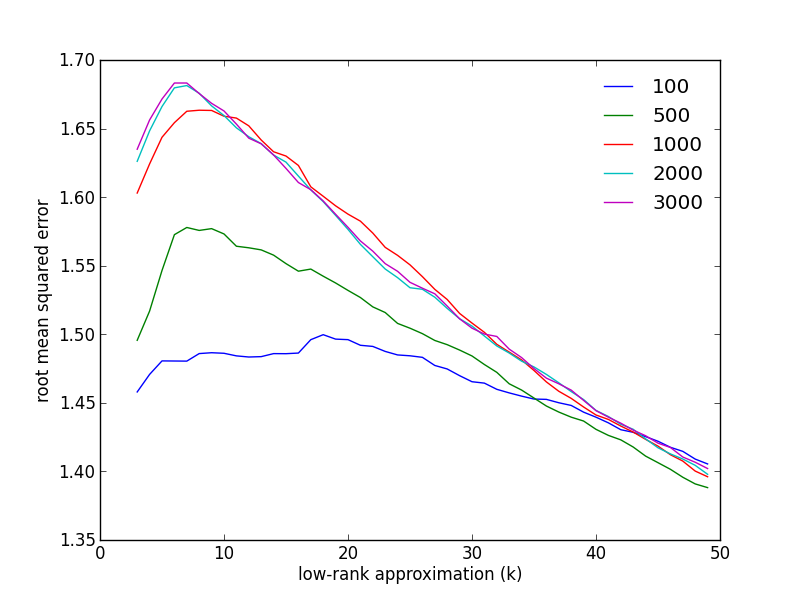
\includegraphics[width=.7\textwidth]{../images/rmse_3000x1000}}
%\fbox{\includegraphics{../scatter_results}}
\end{center}
\caption{RMSE as $k$ increases for several values of $u$ on a 3,000 $\times$ 1,000 subset of the ratings matrix. 10 \% of the ratings are held out for the test set.}
\label{fig:error_small}
\end{figure}

\begin{figure}[H]
\begin{center}
%\framebox[4.0in]{$\;$}
\fbox{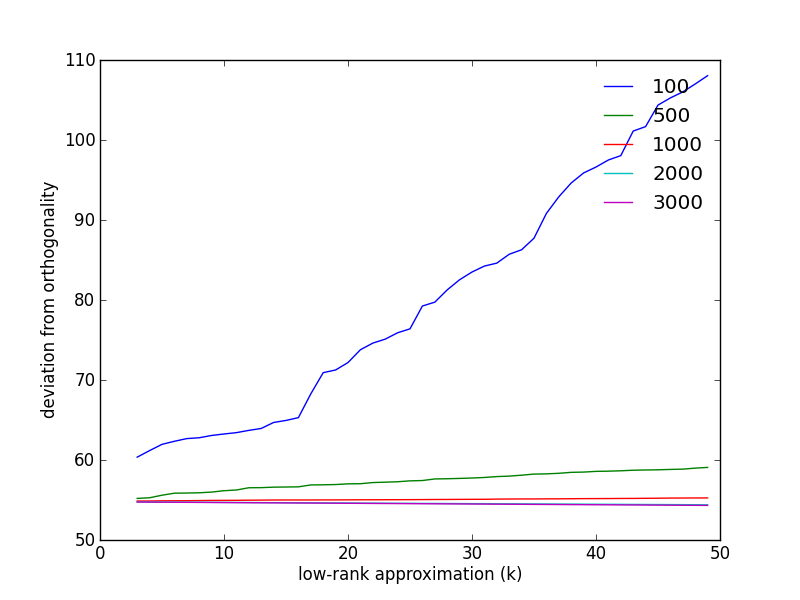
\includegraphics[width=.7\textwidth]{../images/ortho_3000x1000}}
%\fbox{\includegraphics{../scatter_results}}
\end{center}
\caption{Deviations from orthogonality, 
$\|\mathbf{U}_k\mathbf{U}_k^{\T} - \mathbb{I}_m\|_{\textrm{F}}$, for
incremental SVD starting with several different numbers of users.}
\label{fig:ortho_small}
\end{figure}

\section{Conclusion}
In this paper, we created a simple recommendation system by performing incremental SVD on a subset of the ratings matrix used in the Netflix Prize.
In the incremental version, we lose properties of a typical SVD such as orthogonality of the columns (rows) of the $\mathbf{U}$ ($\mathbf{V}$) matrix.
Still, it allows us to implement a recommendation system at scale and to predict user ratings in a satisfactory way.


\bibliography{merity_cook}
\bibliographystyle{plainnat}

\end{document}

